\documentclass[main.tex]{subfiles}
%%------ Preamble specific to this subfile only. This will be used when this document is compiled on its own. When the main document compiles this preabble is ignored. 
%%---------------------------------------------------------------------------%
\begin{document}
\section*{Lesson Plan}

%%------   New command for lesson plan item entries
\begin{comment}
  %Example:
  
  \planItem{5}                %time in minutes
  {Introduction}              % title/name of lesson plan item
  {lesson notes and content}  % this can be a paragraph or a list
  {url}                       % link(s) to resources

\end{comment}

\begin{figure}[h]
  \centering
  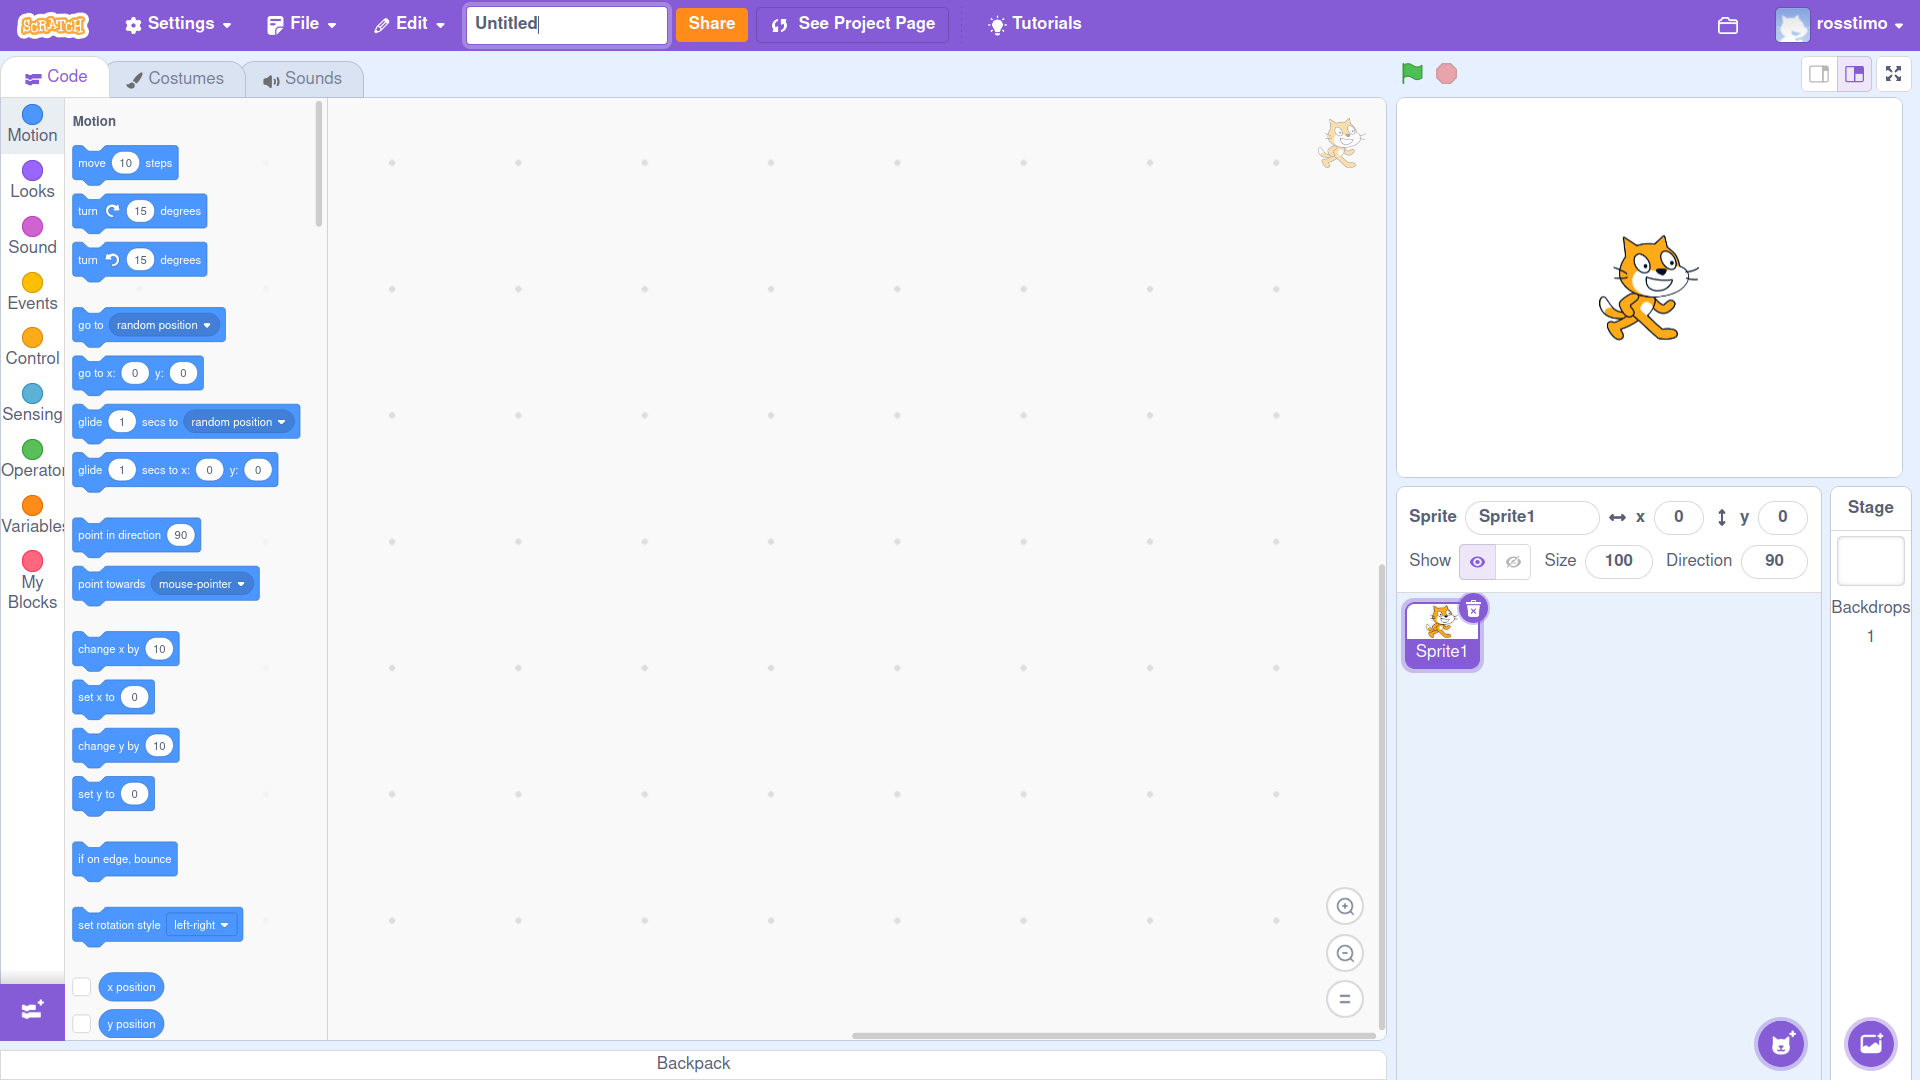
\includegraphics[width=0.8\textwidth]{../images/scratch_interface.png}
  \caption{Scratch Interface}
  \label{fig:scratch_interface}
\end{figure}

\planItem{5}
{Introduction}
{
  The Scratch interface is designed to be user-friendly and intuitive, especially for beginners and children. It allows users to create interactive stories, games, and animations using a visual programming language. Here is an introduction and walk through of the Scratch interface, including its main components and terminology.

}
{\url{https://scratch.mit.edu/}}

\pagebreak[3]

\planItem{10}
{Components of the Scratch Interface}
{
  \begin{enumerate}[label=\textbf{\arabic*.}, leftmargin=2em]
    \item \textbf{Stage} \\
      The Stage is the area where your Scratch project comes to life. It is the backdrop where sprites (characters or objects) perform actions. The Stage uses a 2D coordinate system with \(X\) (horizontal) and \(Y\) (vertical) coordinates to position sprites. The center of the Stage is at coordinates (0, 0).

    \item \textbf{Sprites} \\
      Sprites are the main characters or objects in a Scratch project. Each sprite can have multiple costumes and can be programmed to perform various actions. Sprites are displayed on the Stage and can be controlled using code blocks.

    \item \textbf{Block Palette} \\
      The Block Palette contains all the blocks you can use to create scripts. Blocks are categorized by their functions, such as Motion, Looks, Sound, Events, Control, Sensing, Operators, Variables, and My Blocks. Each category is color-coded for easy identification.

    \item \textbf{Code Area} \\
      The Code Area (or Scripts Area) is where you build your programs by dragging and dropping blocks from the Block Palette. Blocks snap together like puzzle pieces to form scripts, which control the actions of sprites.

    \item \textbf{Sprite Pane} \\
      The Sprite Pane displays all the sprites in your project. You can select a sprite to edit its scripts, costumes, and sounds. The Sprite Pane also allows you to add new sprites from the library, paint your own, or upload images.

    \item \textbf{Toolbar} \\
      The Toolbar at the top of the interface provides options for saving, loading, and sharing projects. It also includes buttons for undoing actions, switching languages, and accessing tutorials.

    \item \textbf{Green Flag and Stop Sign} \\
      The Green Flag is used to start running the scripts in your project, while the Stop Sign stops all running scripts. These controls are located above the Stage.

    \item \textbf{Backpack} \\
      The Backpack is a feature that allows you to store and reuse scripts, costumes, and sounds across different projects. It is located at the bottom of the interface and can be expanded or collapsed as needed.
  \end{enumerate}

}
{\url{https://kicaco.com/what-is-scratch/} \\ \url{https://kicaco.com/sites/default/files/images/scratch\%20editor\%203.jpg}}

\pagebreak[3]


\begin{figure}[h]
  \centering
  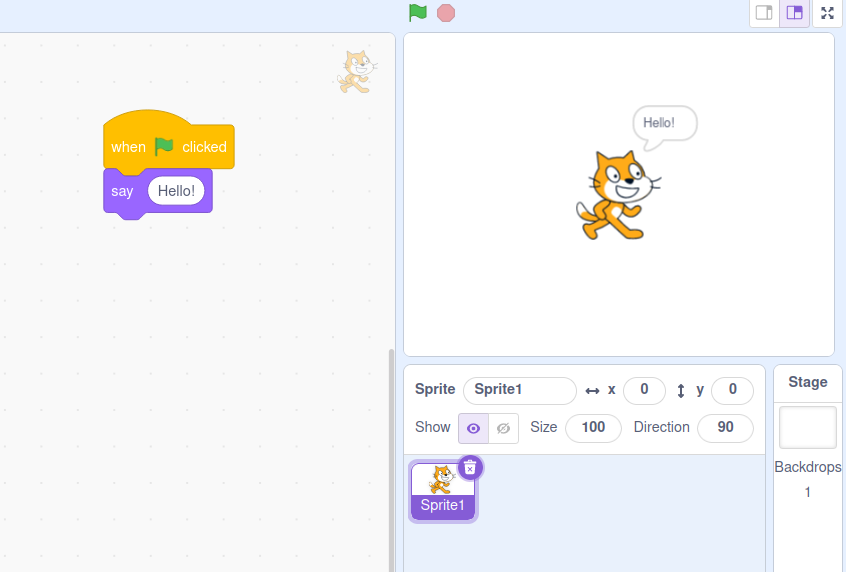
\includegraphics[width=0.8\textwidth, frame]{../images/hello}
  \caption{Hello, Scratchy!}
  \label{fig:scratch_hello}
\end{figure}

\planItem{10}
{Create a Simple Script ``Hello Scratchy"}
{


  \begin{enumerate}[label=\textbf{\arabic*.}, leftmargin=2em]
    \item Click to Select the Scratchy sprite. Or click on the icon to ``Choose a Sprite'' from the library button in the Sprite Pane.
    \item Navigate to the Events category in the Block Palette. (light Orange or Yellow color)
    \item Drag the ``when green flag clicked'' block from the Events category to the Code Area.
    \item Navigate to the Looks category in the Block Palette. (darker Purple color)
    \item Drag the ``say Hello!'' block from the Looks category below the first block.
    \item Click the Green Flag above the Stage to run the script.
    \item Observe the sprite saying ``Hello!'' on the Stage.
  \end{enumerate}
}
{\url{https://scratch.mit.edu/}}

\pagebreak[3]


\planItem{15}
{Main Content}
{\Blindtext [2] [1]}
{www.google.com}

\pagebreak[3]


\planItem{5}
{Activity 2}
{\Blindtext [1] [1]}
{www.google.com}

\pagebreak[3]


\planItem{5}
{Wrap-Up}
{\Blindtext [1] [1]}
{www.google.com}



\end{document}
